\documentclass[a4paper, 10pt]{article}
\usepackage[left=3cm, right=3cm, bottom=3cm, top =3cm]{geometry}
\usepackage[utf8]{inputenc}
\usepackage[slovak]{babel}
\usepackage[IL2]{fontenc}
\usepackage{amsmath}
\usepackage{amsfonts}
\usepackage{amssymb}
\usepackage{graphicx}
\usepackage{color}
\usepackage{booktabs}
\usepackage{wrapfig}
\usepackage[version=3]{mhchem}
%~ \usepackage{auto-pst-pdf}

\usepackage{float}
\newfloat{graph}{h}{graphs}
\floatname{graph}{Graf}
\usepackage{caption}

\usepackage{hyperref}
\usepackage[compact]{titlesec}
\newcommand{\dd}{\ensuremath{ \mathrm{d} }}
\newcommand{\unit}[1]{\ensuremath{\, \mathrm{#1}}}
\newcommand{\di}[1]{\ensuremath{_\mathrm{#1}}}

\begin{document}
\titlespacing{\section}{0pt}{*0}{*0}
\titlespacing{\subsection}{0pt}{*0}{*0}
\titlespacing{\subsubsection}{0pt}{*0}{*0}
\title{Určení krystalové struktury z práškového rentgenového difrakčního záznamu}
\author{Ján Pulmann}
\date{4. 12. 2013}
\maketitle
%%%
\section*{Úlohy}
\begin{enumerate}

	\item Načítajte nameraný záznam, oindexujte ho a nájdite mriežkové parametre.
    \item LeBialovou metódou extrahujte zo záznamu hodnoty štruktúrnych faktorov.
    \item Pomocou vyhasínacích pravidiel nájdite priestorovú grupu hľadanej štruktúry.
    \item Určte počet štruktúrnych jednotiek v elementárnej bunke a pomocou kryštalografických tabuliek nájdite možné polohy atómu v mriežke.
    \item Vyriešte štruktúru látky, tzn. nájdite polohy všetkých atómov v mriežke. Použijte Pattersonovu metódu ťažkého atómu, mapy elektrónových hustôt a Rietveldovu metódu.
    
\end{enumerate}
 %%%
\section*{Teória}

Celá teória čerpá z \cite{stud}.

Kryštalická látka má atómy usporiadané v pravidelnej mriežke. Elementárne bunky tejto mriežky sa nachádzajú na celočíselných súradniciach v báze \textit{mriežových vektorov} základnej bunky.

V troch rozmeroch existuje 14 typov periodických mriežok, ktoré nazývame Bravaisove. Do týchto elementárnych buniek ešte potrebujeme umiestniť atómy. Spolu je týchto spôsobov umiestnenia (ktoré popisujú \textit{priestorové} grupy) 230.

Difrakciu sme čiastočne popísali v predchádzajúcom protokole \cite{predch}. Dôležitý je pre nás reciproký priestor a medzirovinné vzdialenosti v tomto priestore, ktoré súvisia s difrakčnými podmienkami cez \textit{Braggovu rovnicu}. 
\begin{equation}
\label{eq:teor:bragg}
2 d_{hkl} \sin\theta_{hkl} = \lambda\,.
\end{equation}

Z polôh peakov v difrakčnom zázname môžeme určiť tieto vzdialenosti $d_{hkl}$. Z ich hodnôt môžeme pomocou indexovacieho programu určiť typ mriežky a jej mriežkové parametre (rozmery elementárnej bunky)

Z hustoty, sumárneho vzorca a rozmerov elementárnej bunky môžeme určiť, kolko atómov sa nachádza v elementárnej bunke. 

Na určenie hmotnej bázy použijeme intenzity nameraných peakov. Amplitúdy žiarenia popisuje \textit{štrutkúrny faktor}
\begin{equation}
\label{eq:teor:strukturny_faktor}
F_{hkl} = \sum_{j=1}^n f_j e^{-i\bold{q}\cdot \mathbf{r_j}}\,,
\end{equation}
kde $f_j$ je atómový rozptylový faktor (môžeme aproximovať počtom elektrónov), $\mathbf{r_j}$ sa pohybuje po polohách atómov a $\mathbf{q}$ je rozdiel vlnových vektorov dopadajúcej a odrazenej vlny. Pre rozptyl na rovine určenej indexami $hkl$ potom definujeme $F_{hkl}$.

Pattersonovu funkciu definujeme z elektrónovej hustoty $\rho$ vzťahom 
\begin{equation}
\label{eq:teor:patterson}
P(x) = \frac 1a \int_0^a \rho(x')\rho(x'-x)\dd x\,.
\end{equation}

Štruktúrny faktor je pôvodne definovaný ako Fourierova transformácia hustoty elektrónov, po dostadení jeho inverznej transformácie do Pattersonovej funkcie dostaneme vzťah na jej výpočet z veľkostí štruktúrnych faktorov
\begin{equation}
\label{eq:teor:patterson_z_Fhkl}
P(x, y, z) = \frac{1}{V^2}\sum_h \sum_k \sum_l |F_{hkl}|^2\cos[2\pi (hx + ky + lz)]\,,
\end{equation}

$|F_{hkl}|^2$ môžeme určiť z intenzít peakov vzťahom 15 v \cite{stud}.
Metóda fitovania peakov bez ohľadu na šturkúru nazývame bezštruktúrnou Rietveldovou metódou či LeBailovým fitovaním. 

Priestorovú grupu určíme z vyhasínacích pravidiel, porovnaním s výsledkom LeBailovým fitovaním.

Na určenie polôh atómov budeme fitovať vygenerovaný difrakčný záznam podľa rôznych parametrov do nameraného záznamu. Zadané parametre upravujeme napr. metódou najmenších štvorcov. Potrebujeme špecifikovať mriežkové parametre, priestorovú grupu, polohy atómov v mriežke a parametre merania ako polohy vlnovú dĺžku, typ žiarenia a napr. použitie monochromátoru.

%%%
\section*{Postup merania}
Postup merania sme popísali v teórii, špecifiká experimentu popíšeme vo výsledkoch merania.
\subsection*{Pomôcky} difrakčný záznam, program(y) \texttt{FullProf} , kryštalografické tabuľky
%%%
\section*{Výsledky merania}
Nameraný difrakčný záznam je v grafe \ref{graph:spektrum}. Tento záznam bol nameraný s použitím monochromátoru, takže pozorujeme len dve čiary medi, $K_{\alpha 1,\, 2}$. Ďalej opíšeme jednotlivé kroky podrobnejšie s číselnými výsledkami.

\begin{itemize}
\item Automaticky nájdeme peaky pomocou voľby \texttt{Points Selection/Automatic peak search}. Volíme dublet čiar $K_\alpha$ pre meď. Nájdené peaky uložíme pre nasledujúci program. 
\item Ďalej sa pokúsime určiť Bravaisovu mriežku našej látky. Použijeme program \texttt{DICVOL}, kde si môžeme pri ukladaní nájdených peakov rôzne mriežky. Sledujeme mriežkové parametre a dve čísla udávajúce kvalitu fitu, \texttt{M(N)} a \texttt{F(N)} - čím vyššie, tým lepšie.

Medzi možných kandidátov patria tetragonálna, hexagonálna a ortorombická mriežka. Ortorombická mriežka má ale veľmi podobné parametre ako tetragonálna - zhoda na 4 platných cifriach, \texttt{DICVOL} teda zrejme našiel tú istú sústavu. V hexagonálnej máme oveľa nižšie \texttt{M(N)} a \texttt{F(N)}, rozhodli sme sa teda pokračovať s tetragonálnou sústavou. Jej parametre sú

\begin{align*}
a&=4.0139 \unit\AA  \\
b&=4.0139 \unit\AA  \\
c &= 13.0917 \unit\AA \\
V &= 210.92 \unit\AA ^3\\
M(N) &= 169.9 \\
F(N) &= 114.9
\end{align*}

Zaujímavé v tomto kroku bolo, že programu stačilo len 20 z 47 nájdených peakov. 

\texttt{DICVOL} vypíše formát \texttt{.pcr}, s ktorým budeme ďalej pracovať.

\item Z hustoty látky $3.35 \unit{g\cdot cm^{-3}}$ a molekulovej hmotnosti vieme určiť, že v elementárnej bunke by sa mali nachádzať dve molekuly $\ce{K2NiF4}$.

\item Ďalej zistíme hodnoty intenzít na určenie štruktúrnych faktorov. Vezmeme najvšeobecnejšiu grupu symetrie tetragonálnej látky s danými mriežkovými parametrami a prekladáme vygenerovaným záznamom ten nameraný. Uvidíme, že niektoré peaky sú oveľa nižšie ako by mali byť a pokúsime sa odhadnúť všeobecný vzor $hkl$.

V našom prípade zistíme, že ide o $h+k+l = 2n$, čo je podľa \cite{tab} telesovo centrovaná priestorová grupa bez ďalších sklzových rovín - teda $I/4mmm$ \footnote{rozumiem tomu tak, že sme vybrali najväčšiu grupu, ktorá je tetragonálna, telesovo centrovaná atp. Má samozrejme telesovo centrované podgrupy. Jej telesovo centrovaná nadgrupa je $Im\bar{3}m$, ktorá je ale kubická - čo vieme, že nie je náš prípad z určenia mriežkových parametrov.}.

Pri tomto postupe editujeme súbor \texttt{.pcr} a spúšťame \texttt{FullProf}. Ide o metódu najmenších štvorcov, kde funkcia je simulácia difrakčného r\"ontgenového merania a namerané hodnoty je difrakčný záznam. Môžeme si voliť, ktoré parametre používame a tiež ich navzájom obmedzene korelovať - pri fitovaní mriežkového parametra $a$ napr. fitujeme len 1 hodnotu, aj keď je v súbore dva krát.
Používame parametre \texttt{U}, \texttt{V}, \texttt{W}, ktoré upravujú šírku peakov ako kvadratickú funkciu od $2\theta$, \texttt{Bov} popisujúci tepelný pohyb atómov, mriežkové parametre a parametre popisujúce tvar peakov, \texttt{Scale} a \texttt{Shape1}.


\item Teraz sa môžeme prvý kráť pozrieť na výstup Pattersonovej funkcie. Urobíme to programom \texttt{GFourier}, ktorý načítava súbor \texttt{.inp} (ten bol vygenerovaný pri prekladaní nameraného záznamu \texttt{FullProf}om). Zvolíme metódu \texttt{Fobs Patterson}. 

Hľadáme najvyššiu intenzitu, pretože zrejme pôjde o najťažší Nikel. Ďalšiu informáciu zistíme z \cite{tab}. V elementárnej bunke budú 2 atómy $\ce{Ni}$. Uvádzame kúsok tabuľky z \cite{tab}, v stĺpcoch sú postupne multiplicita, Wyckoffove písmeno a možné polohy atómov. Okrem uvedených polôh každej polohe prislúchajú aj súradnice zväčšené o vektor $(\frac 12,\frac 12,\frac 12)$, pričom počítame modulo 1 v intervale $\texttt{[0, 1)}$.
\begin{align*}
\texttt{2} \;\;\;& \texttt{b} \;\;\;  \texttt{0,0,} \frac {\texttt{1}}{\texttt{2}} \\
\texttt{2} \;\;\;& \texttt{a} \;\;\;  \texttt{0,0,0}
\end{align*}

Keďže silné intenzity pre autokorelačnú funkciu (obrázky \ref{graph:rez0} a \ref{graph:rez1/2}) vidíme v $(0,0,0)$ a v  $(\frac 12,\frac 12,\frac 12)$, ide zrejme o Wyckoffove písmeno \texttt{a}.

Do \texttt{.pcr} súboru teda pridáme riadok 
\begin{verbatim}
!Atom   Typ       X        Y        Z     Biso       Occ     In Fin N_t Spc /Codes
Ni     NI+2    0.00000  0.00000  0.00000  0.00000   2.00000   0   0   0    0  
\end{verbatim}
FullProf už sám vie, že má pridať aj atóm niklu do stredu ($2\times \texttt{Occ}$). 
Opäť spustíme FullProf, trochu sa nám vylepší zhoda a môžeme ďalej skúmať autokorelačnú funkciu.

\item Pokračujeme v hľadaní atómov, teraz sa snažíme umiestniť štyri draslíky. Pre tie vyberáme polohu s multiplicitou 4, keďže tie s multiplicitou sú bez parametra a jedna je už zabratá niklom. Nebudeme už prepisovať \cite{tab}, z grafov \ref{graph:rezy0} a \ref{graph:rezy1/2} určíme, že ide o polohu $(0,0,z)$, $(0,0,-z)$ (\texttt{e}). Intenzity v týchto rezoch sú intenzity ukázané v oveľa menšom rozsahu. Pri meraní sme chybne určili $z\approx 0.17$, čo sa neskôr ukázalo ako poloha fluórového atómu. Napriek tomu sa nám podarilo dofitovať a až neskôr sme zistili správnu polohu $z\approx 0.35$. Pri spätnom pohľade na elektrónové hustoty to už vyzerá zrejmé\footnote{Počas merania som bol zmätený a nepochopil som, že $\bar z = -z$, myslel som si $\bar z = \frac 12 -z$, čo mohlo byť zdrojom chyby}.

\item Nakoniec určíme polohy fluórov. Sú čiastočne viditeľné na grafoch s rezom v $y$. Opäť hľadáme buď dve polohy s multiplicitou 4 alebo jednu s multiplicitou 8. Použili sme rozmiestnenie \texttt{e},   $(0,0,z)$ s $z\approx 0.15$ a \texttt{c} s polohami  $(0,\frac 12, 0)$ a  $(\frac 12,0,0)$\footnote{ Tú druhú polohu teraz síce veľmi nevidím v elektrónovej hustote, no stále mohla byť prekrytá ostatnými atómami. Fluór má tiež záporný náboj, čo by mohli byť práve miesta so zápornou hustotou. Výsledná prekladaná štruktúra súhlasí s nameraným spektrom}.

Po preložení s množstvom parametrov (popísaných vyššie, navyše fitujeme aj polohy atómov $z$) dostaneme výsledok s kvalitou
\begin{verbatim}
    =>    Bragg R-factor:   2.747
    =>    RF-factor     :   3.557
\end{verbatim}
pričom sme začínali s hodnotami okolo 70 a 90 pri iba niklovom atóme. Dosiahli sme podobné hodnoty ako pri prekladaní bez ohľadu na štruktúru. Preložená závislosť a rozdiel je  v grafe \ref{graph:vse}. 

\item Štruktúru vykreslíme   v programe \texttt{FullProf Studio} do obrázku \ref{image:vysl} (obrázok bol potom ďalej upravený kvôli problémom s exportom). Jednotlivé atómy a ich polohy sú farebne odlíšené.

Výsledné mriežkové parametre sú 
\begin{align*}
 a =b &= 4.013071\unit\AA  \,, \\
 c &= 13.088236 \unit\AA \,.
\end{align*}
\end{itemize}

\begin{graph}[tb]
\centering
%~ \vspace*{-15pt}
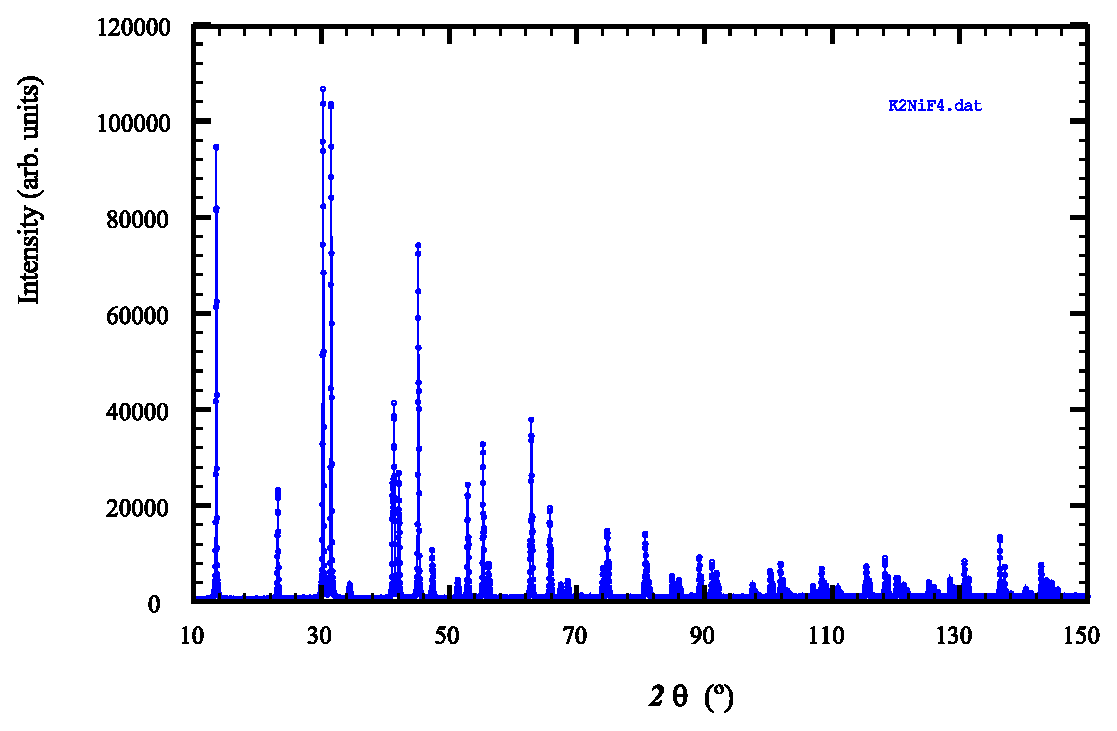
\includegraphics[scale=0.70]{data/spektrum.eps}
%~ \vspace*{-10.2cm}
\caption{ Práškový difrakčný záznam \label{graph:spektrum}}
\end{graph}

%%%
\section*{Diskusia}
Postup bol výrazne uľahčený množstvom programov na jednotlivé kroky. Celý obsah úlohy A19 sme vlastne zvládli za približne 5 minúť. Programy na seba ale nie vždy úplne naväzujú a každý obsahuje vlastný spôsob, ako zadávať vstup (rôzne vstupné súbory, kódy v \texttt{.pcr} súboroch na určovanie fitovania) - rekunštruovať postup po meraní bolo náročné a niektoré kroky sa mi nepodarili úplne presne.

Kvalita nameraného difrakčného záznamu bola dostatočná pre spracovanie, dostávali sme sa už na limit modelu pri fitovaní.

Určovanie polôh hlavne fluóru bolo náročné, do základnej bunky zasahuje 22 atómov F. Umiestnenie do polohy \texttt{e} (zelenomodré atómy v obr \ref{image:vysl}) bolo dobre odhadnuteľné, no to do polohy \texttt{c} (fialové atómy v \ref{image:vysl}) už horšie. Neviem nakoľko je zhod generovaného záznamu s nameraných rozhodujúci, u nás je zhoda dobrá, hoci nie dokonalá.
%%%
\section*{Záver}
Pre $\ce{K2NiF4}$ sme Bravaisovu mriežku - tetragonálnu, priestorovú grupu - $I/4mmm$ a mriežkové parametre
\begin{align*}
 a =b &= 4.013071\unit\AA  \,, \\
 c &= 13.088236 \unit\AA \,.
\end{align*}
Ďalej sme študovali elektrónové hustoty (grafy \ref{graph:rez0}, \ref{graph:rez1/2}, \ref{graph:rezy0}, \ref{graph:rezy1/2}) a určili sme polohy jednotlivých atómov v elementárnej bunke:
\begin{itemize}
\item pre nikel sú to $(0,0,0)$ a prislúchajúca $(\frac 12,\frac 12,\frac 12)$ (tú už nebudem ďalej uvádzať).
\item pre draslík je to $(0,0,z)$ a $(0,0,-z)$ (+ pričítané  $(\frac 12,\frac 12,\frac 12)$) s $z=0.35388$
\item a pre fluór máme dve polohy, \\
    $(0,\frac 12, 0)$, $(\frac 12,0,0)$ \\
    a $(0,0,z)$, $(0,0,-z)$ s $z=0.15323$.
\end{itemize}
Nakoniec sme štruktúru vizualizovali zakreslením polôh týchto atómov do obrázku \ref{image:vysl}

%%%
\begin{thebibliography}{9}

\bibitem{stud}
    \emph{Študijný text ku úlohe A22} \\
    \url{http://krystal.karlov.mff.cuni.cz/kfes/vyuka/lp/
} 18.11.2013

\bibitem{tab}
    Hahn, Theo \textit{International Tables for Crystallography}, 5. ed (Springer, Dordrecht 2005)

\bibitem{predch}
    Pulmann, Ján \textit{Protokol k úlohe A19} {\tiny umiestnený na} \\{\footnotesize \mbox{\url{https://github.com/jpulmann/praktikum/blob/master/PraktikumIV/praskova_difrakcia_A19/ulohaA19.pdf}}}
\end{thebibliography}


\begin{graph}[tb]
\centering
\hspace*{-78pt}
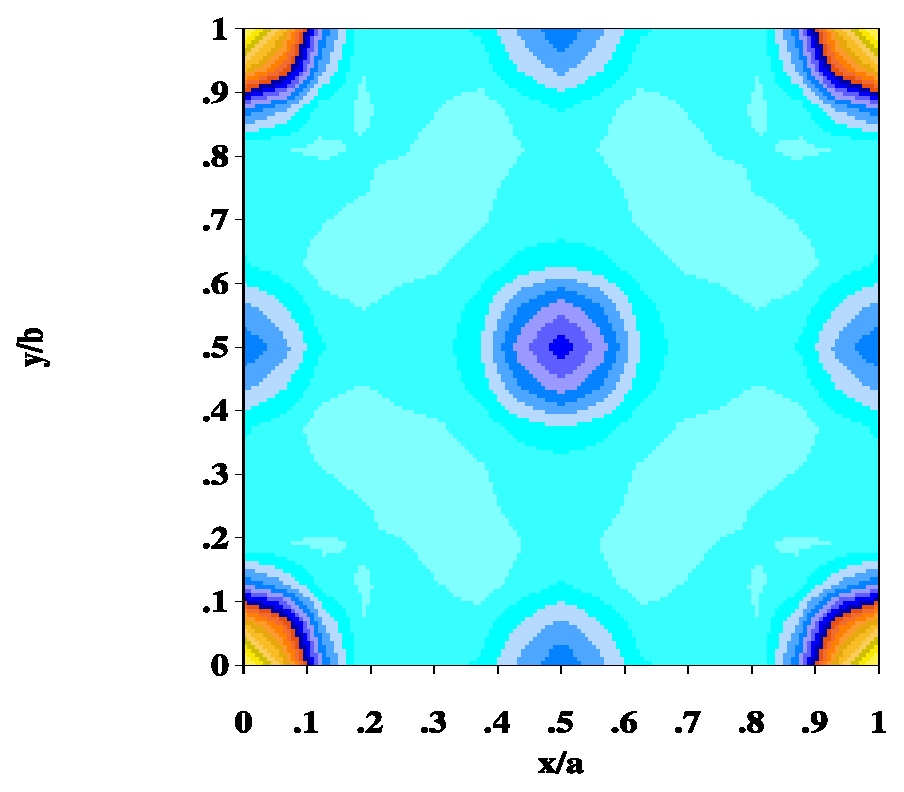
\includegraphics[scale=0.8]{data/k2nif4_1.eps}
%~ \vspace*{-10.2cm}
\caption{ Rez autokorelačnou funkciou pre $z=0$ \label{graph:rez0}}
\end{graph}

\begin{graph}[tb]
\centering
\hspace*{-78pt}
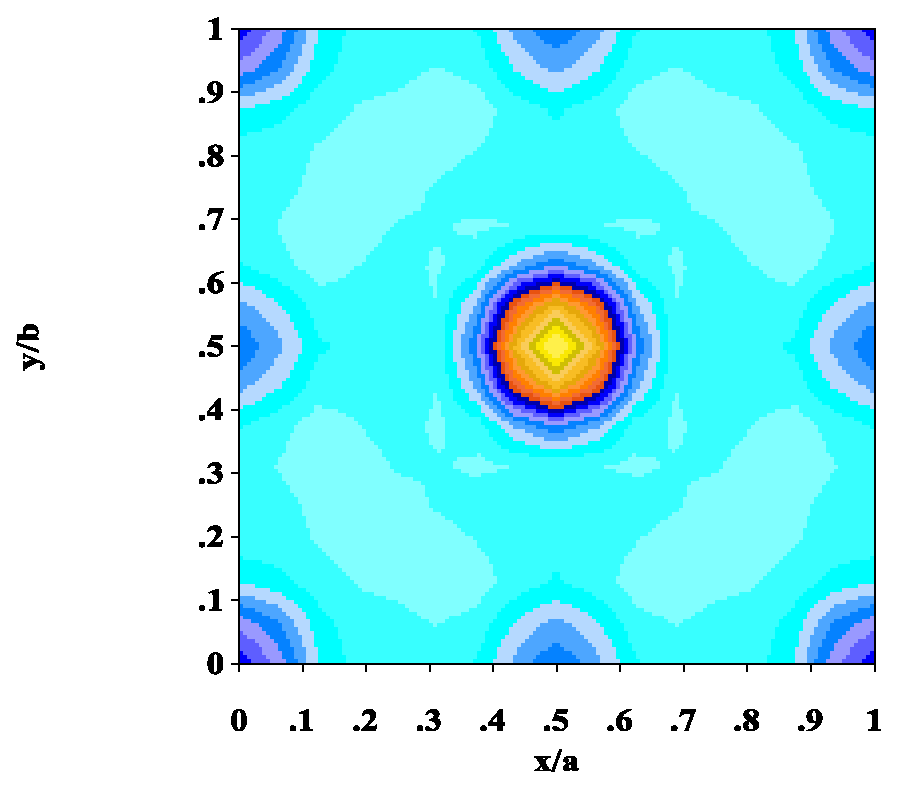
\includegraphics[scale=0.8]{data/k2nif4_1z0_5.eps}
%~ \vspace*{-10.2cm}
\caption{ Rez autokorelačnou funkciou pre $z=1/2$ \label{graph:rez1/2}}
\end{graph}


\begin{graph}[tb]
\centering
\hspace*{-40pt}
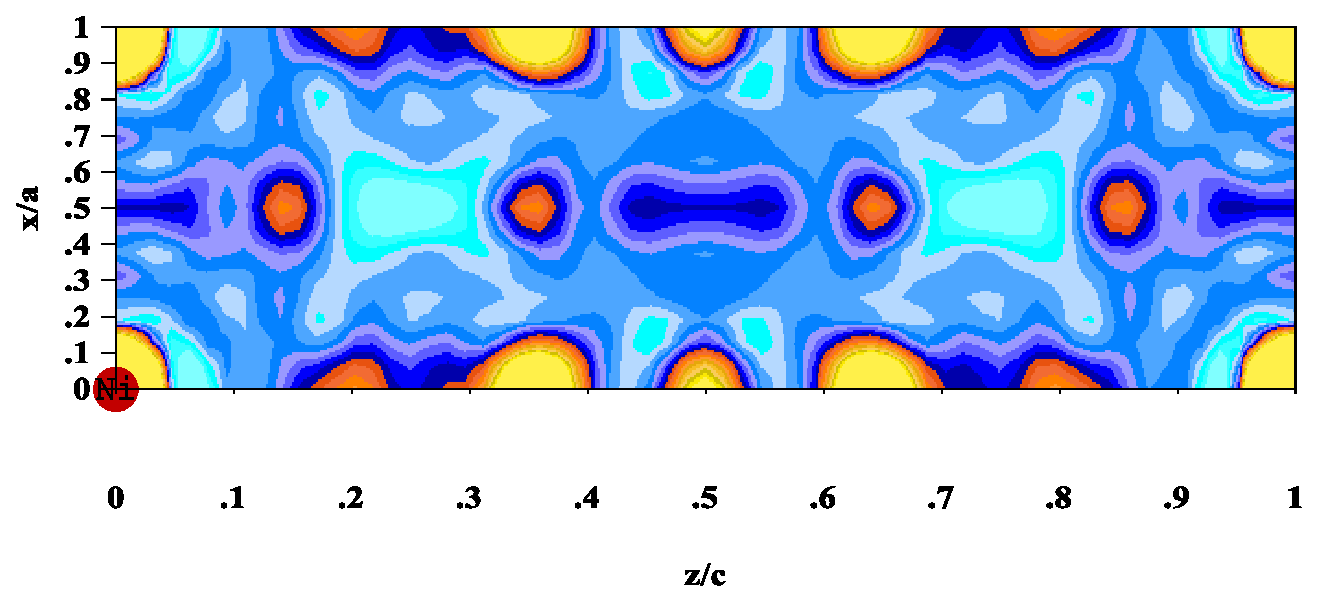
\includegraphics[scale=0.8]{data/k2nif4y_0.eps}
%~ \vspace*{-10.2cm}
\caption{ Rez autokorelačnou funkciou pre $y=0$ \label{graph:rezy0}}
\end{graph}

\begin{graph}[tb]
\centering
\hspace*{-40pt}
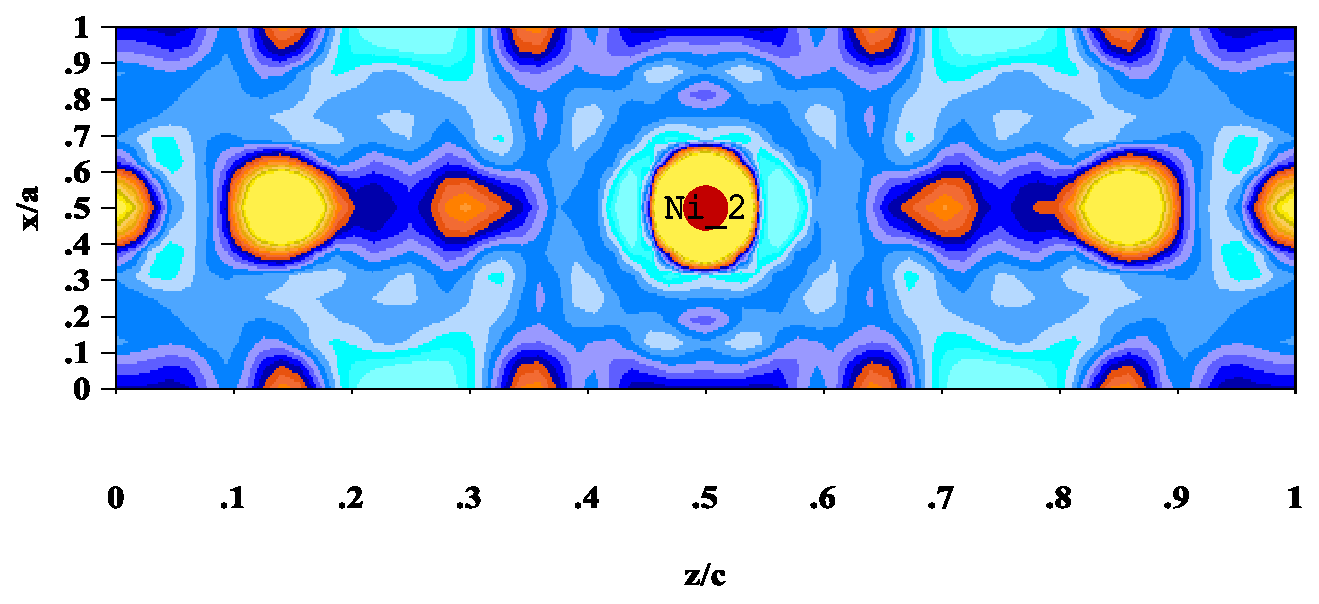
\includegraphics[scale=0.8]{data/k2nif4y_05.eps}
%~ \vspace*{-10.2cm}
\caption{ Rez autokorelačnou funkciou pre $y=1/2$ \label{graph:rezy1/2}}
\end{graph}


\begin{graph}[tb]
\centering
%~ \vspace*{-15pt}
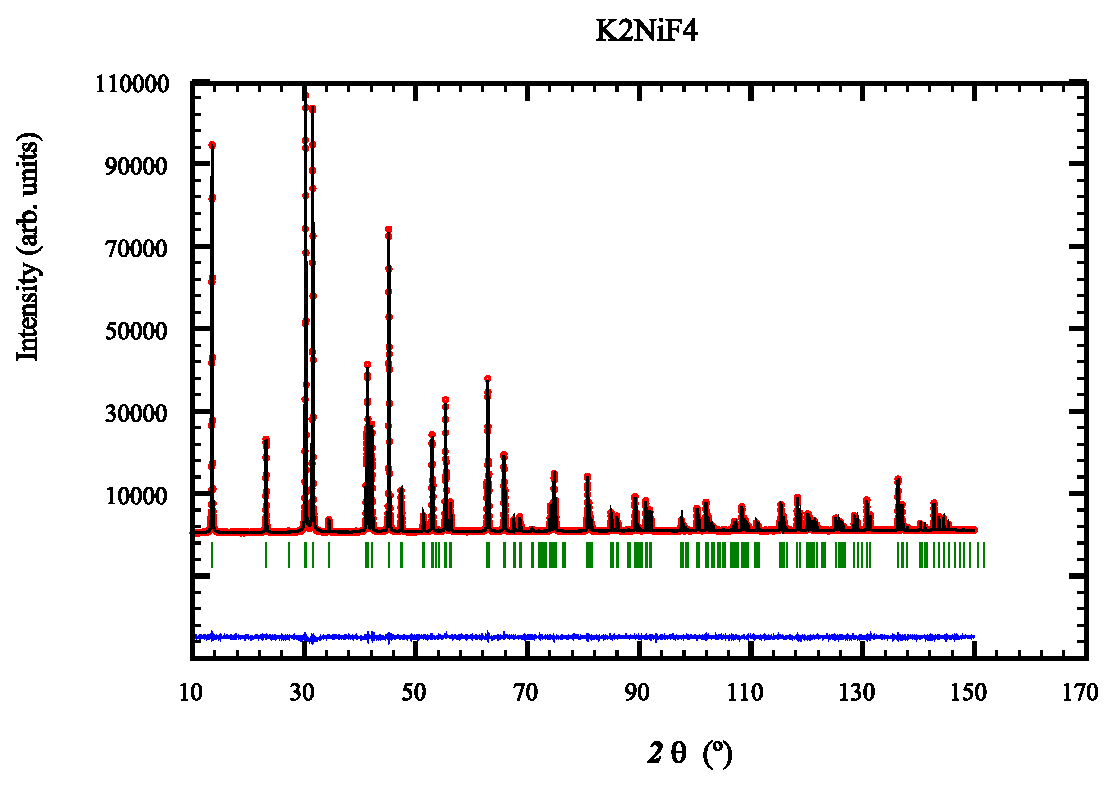
\includegraphics[scale=0.70]{data/vse.eps}
%~ \vspace*{-10.2cm}
\caption{ Práškový difrakčný záznam a fit na základe určenej kryštálovej štruktúry\label{graph:vse}}
\end{graph}

\begin{figure}[tb]
\centering
%~ \vspace*{-15pt}
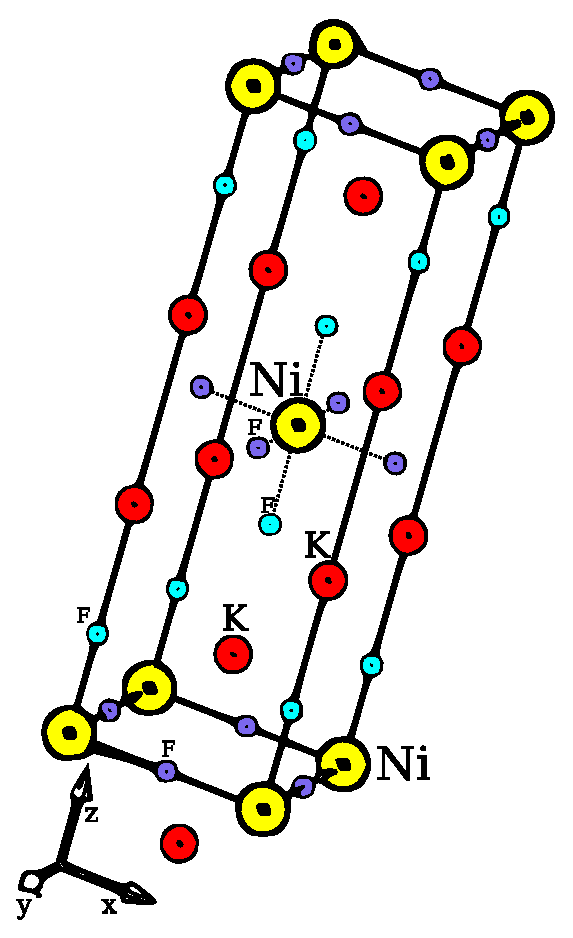
\includegraphics[scale=1.5]{data/vysl.eps}
%~ \vspace*{-10.2cm}
\caption{ Výsledná štruktúra $\ce{K2NiF4}$ \label{image:vysl}}
\end{figure}

\end{document}
